\begin{landscape}
\section{Anhang}
\subsection{Diverse Formeln bzgl. Magnetismus} \label{seich}
\begin{tabular}{llll}
  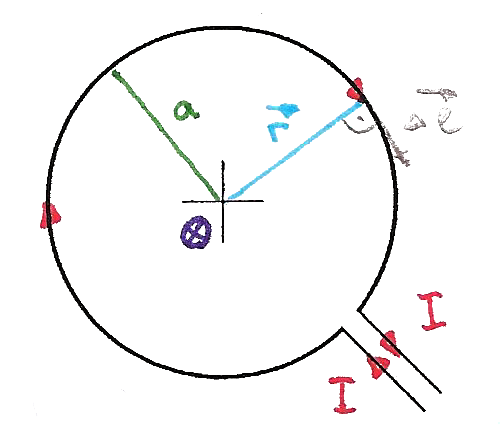
\includegraphics[width=5.7cm]{./pics/biot1.png} &
  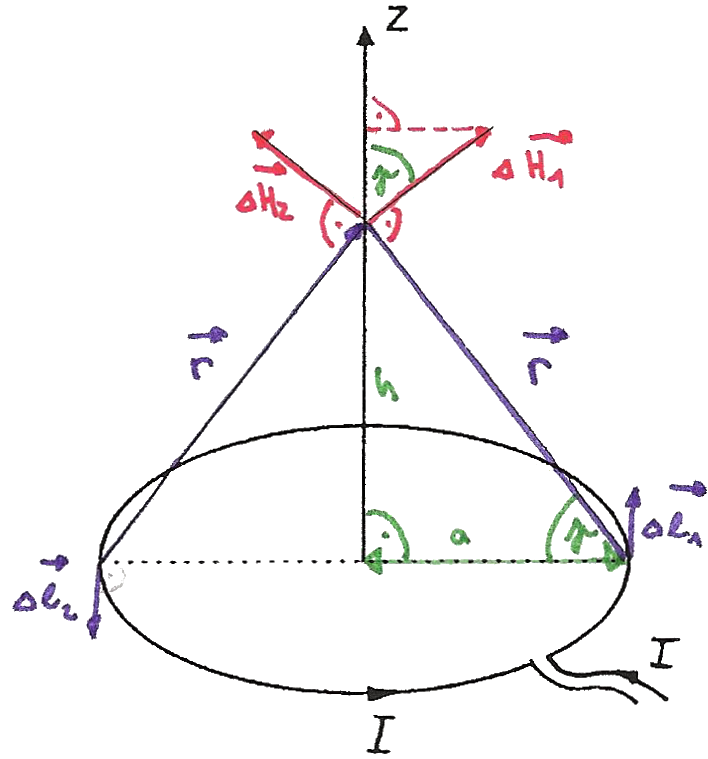
\includegraphics[width=5.7cm]{./pics/biot2.png} &
  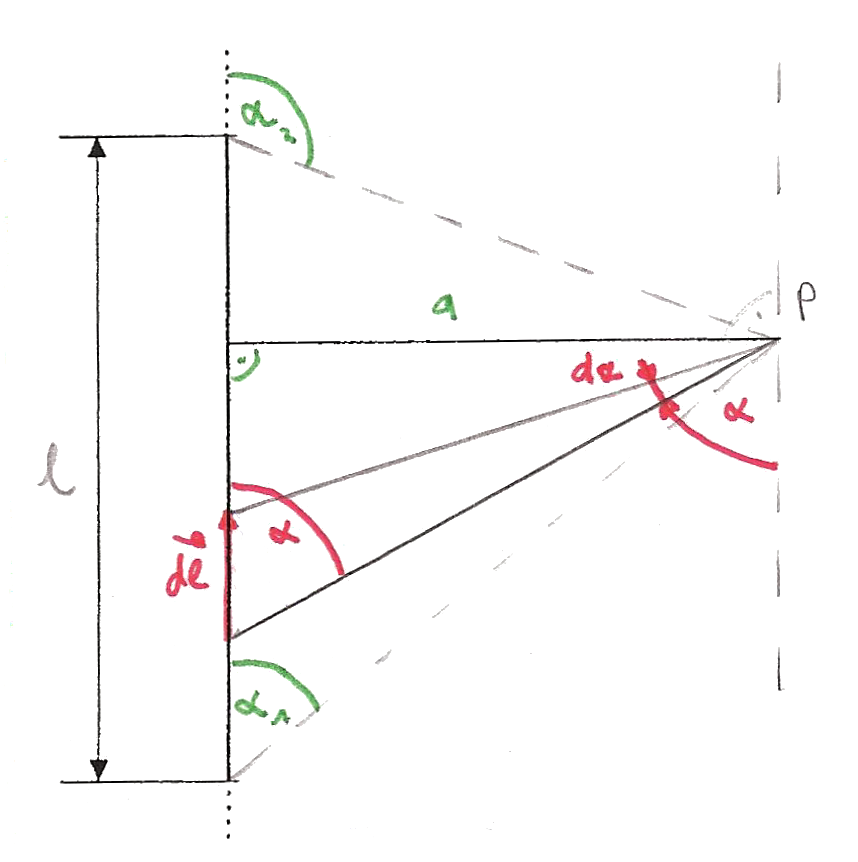
\includegraphics[width=5cm]{./pics/biot3.png} &
  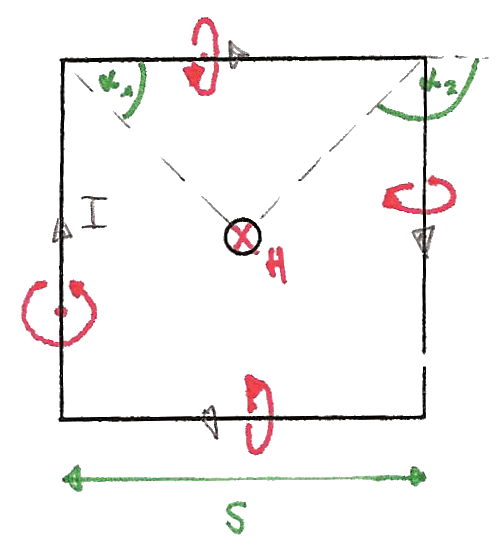
\includegraphics[width=5.7cm]{./pics/biot4.png} \\
  $H =\frac{I}{D} = \frac{I}{2a}$ &
  $H=\frac{I}{2} \cdot \frac{a^2}{\sqrt{a^2+h^2}^3}$ &
  $H=\frac{I}{4\pi a}(\cos(\alpha_1)- \cos(\alpha_2))$ &
  $H= \frac{I \cdot 2 \sqrt{2}}{\pi \cdot s}$ \\
\end{tabular}

\subsection{Ferromagnetische Stoffe} \label{ferromagnetische_stoffe}
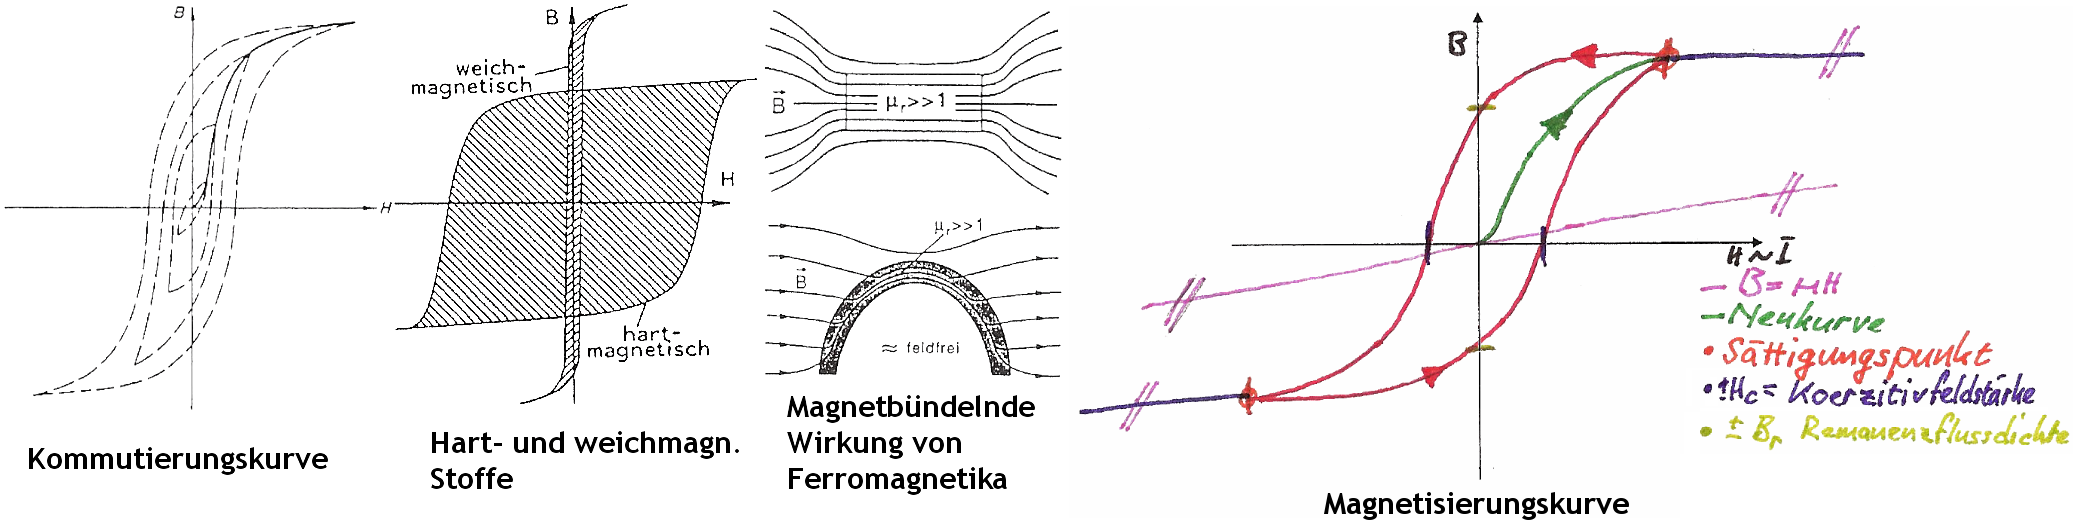
\includegraphics[width=25cm]{./pics/magnetisierung.png}

\end{landscape}